% section 3

\section{環境識別子とその精密化}

\kam{ここに須藤研究と大石研究の図をいれる(大石研究の図は、次の章に移動
  する予定だが、とりあえず、ここにいれておいてください)}

\begin{center}
  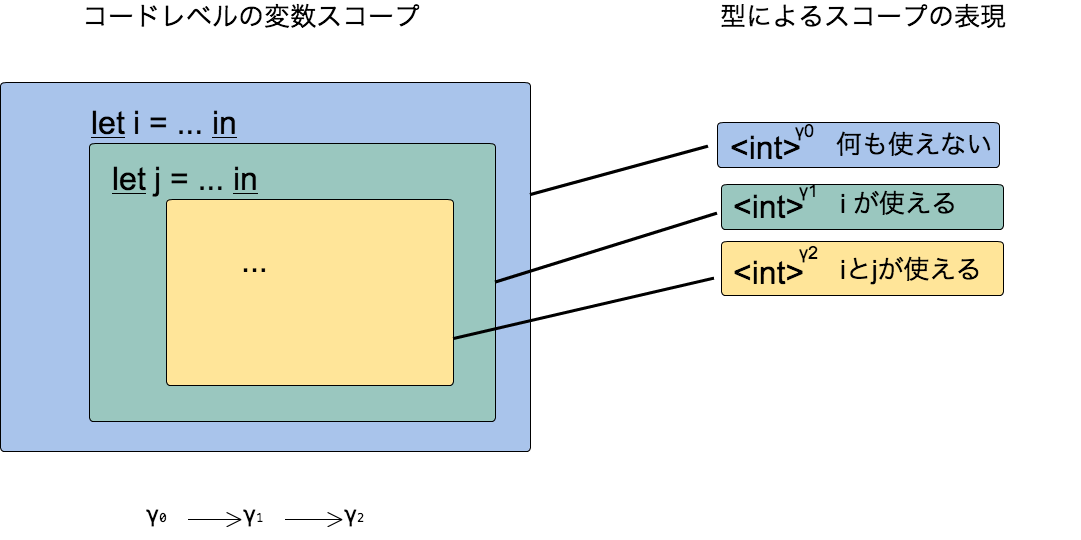
\includegraphics[clip,height=4cm]{./img/ec_let.png}
\end{center}

\begin{center}
  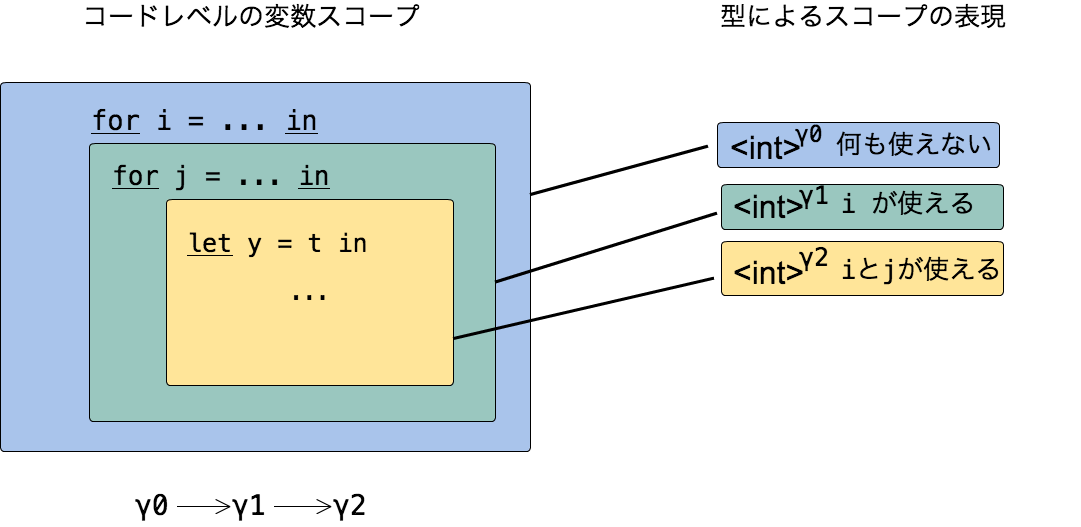
\includegraphics[clip,height=4cm]{./img/ec_for.png}
\end{center}

% \begin{tikzpicture}
%   \node (s) {$\gamma_0$};
%   \node[above right=of s] (a) {$\gamma_1$};
%   \node[below right=of s] (b) {$\gamma_2$};
%   \node[below right=of a] (t) {$\gamma_3 = \gamma_1 \cup \gamma_2$};

%   \foreach \u / \v in {s/a,s/b,b/t,a/t}
%   \draw[->] (\u) -- (\v);
% \end{tikzpicture}

\begin{center}
  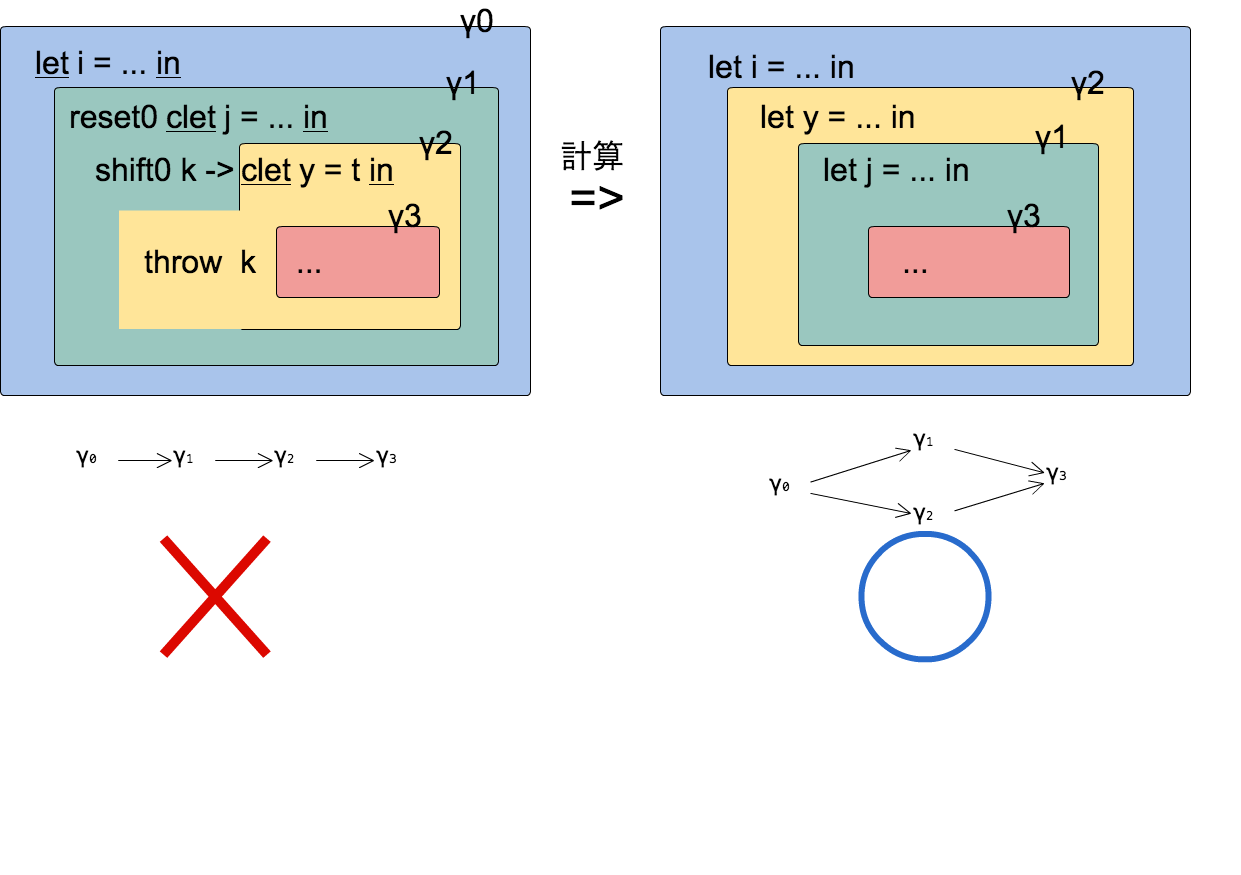
\includegraphics[clip,height=5.5cm]{./img/ecex_let.png}
\end{center}

\begin{center}
  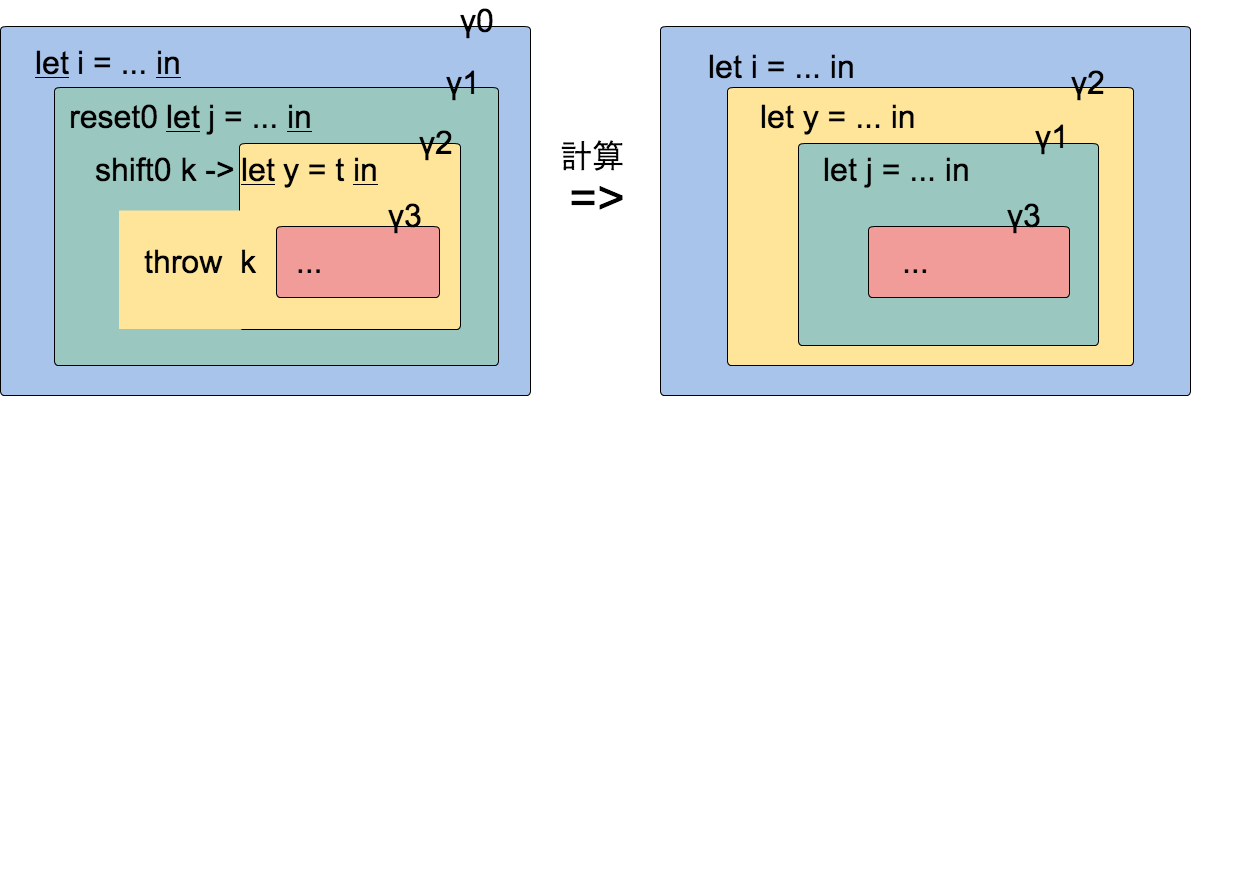
\includegraphics[clip,height=5.5cm]{./img/ecex_let_non_gamma.png}
\end{center}

\begin{center}
  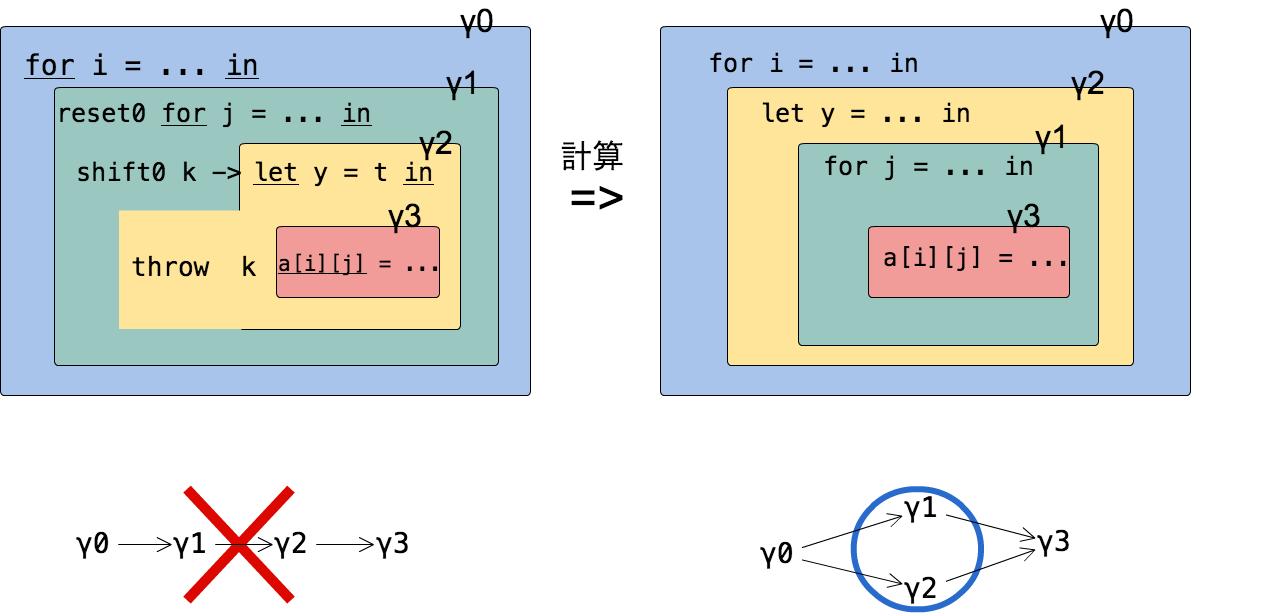
\includegraphics[clip,height=4cm]{./img/ecex_for.png}
\end{center}

\begin{center}
  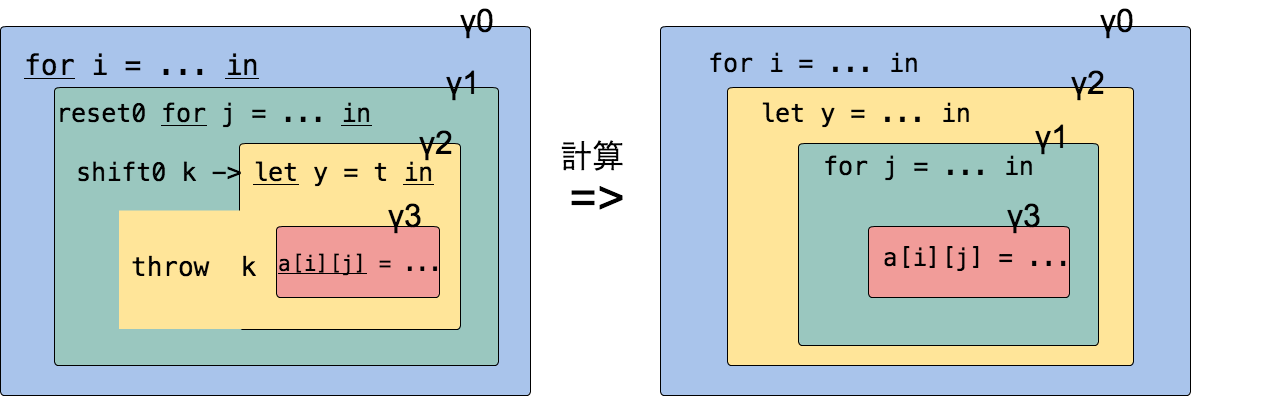
\includegraphics[clip,height=3cm]{./img/ecex_for_non_gamma.png}
\end{center}

\begin{center}
  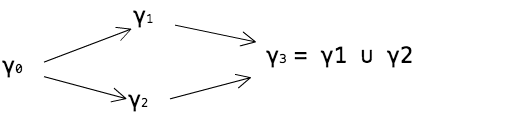
\includegraphics[clip,width=7cm]{./img/gamma.png}
\end{center}

\begin{center}
  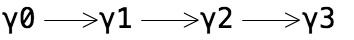
\includegraphics[clip,width=4cm]{./img/gamma_normal.png}
\end{center}

%%% Local Variables:
%%% mode: japanese-latex
%%% TeX-master: "paper"
%%% End:
